\documentclass[11pt]{standalone}
\usepackage{amssymb}
\usepackage{amsmath}
\usepackage[no-math]{fontspec}
\usepackage{unicode-math}
\usepackage{libertinus}
\usepackage{pgf,xcolor}
\usepackage{tikz}
\usetikzlibrary{arrows.meta, backgrounds, calc}
\usepackage{pgfplots}
\pgfplotsset{compat=newest}

% ── Color palette (all seven defined in every file) ──────────────────────────
\definecolor{my_darkgray}{HTML}{484949}
\definecolor{my_lightgray}{HTML}{F3F4F4}
\definecolor{my_darkblue}{HTML}{005A94}
\definecolor{my_lightblue}{HTML}{CCDEE9}
\definecolor{my_yellow}{HTML}{FFEC7F}
\definecolor{my_red}{HTML}{E60000}
\definecolor{my_orange}{HTML}{E87846}

\begin{document}
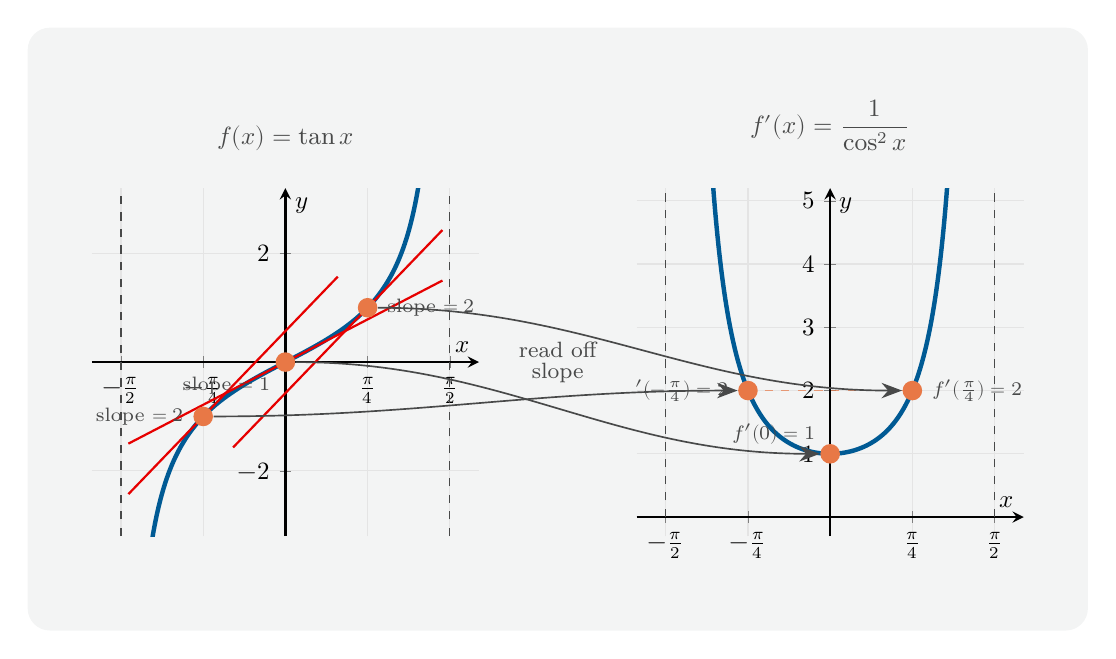
\begin{tikzpicture}[
    show background rectangle,
    background rectangle/.style={fill=my_lightgray, rounded corners=8pt},
    inner frame sep=0.8cm
]

% ── Left panel: f(x) = tan(x), central branch, tangent lines at -π/4, 0, π/4 ─
%
% Only the central branch of tan(x) is shown. Vertical asymptotes at x = ±π/2
% are drawn as dashed lines. axis equal omitted: y range [-3, 3] against
% x range [-1.8, 1.8] would make the panel too narrow at equal scale.
%
\begin{axis}[
    name             = ax_left,
    width            = 6.5cm,
    height           = 6.0cm,
    axis lines       = center,
    xlabel           = {$x$},
    ylabel           = {$y$},
    grid             = both,
    grid style       = {color=my_darkgray!15},
    xmin = -1.85,  xmax = 1.85,
    ymin = -3.2,   ymax = 3.2,
    axis line style  = {thick},
    title            = {$f(x) = \tan x$},
    title style      = {font=\small\bfseries, color=my_darkgray, yshift=4pt},
    tick label style = {font=\small},
    label style      = {font=\small},
    xtick            = {-1.5708, -0.7854, 0, 0.7854, 1.5708},
    xticklabels      = {$-\tfrac{\pi}{2}$, $-\tfrac{\pi}{4}$,
                        $0$, $\tfrac{\pi}{4}$, $\tfrac{\pi}{2}$},
    ytick            = {-2, 0, 2},
]

  % Asymptotes at x = ±π/2 drawn first so the curves sit on top.
  \pgfplotsextra{
    \draw[color=my_darkgray, dashed, thin]
        (axis cs:-1.5708, -3.2) -- (axis cs:-1.5708, 3.2);
    \draw[color=my_darkgray, dashed, thin]
        (axis cs: 1.5708, -3.2) -- (axis cs: 1.5708, 3.2);
  }

  % Central branch of tan(x).
  % pgfplots trig functions use degrees; wrap x in deg() for radians.
  % Domain stops 0.07 rad short of ±π/2 ≈ ±1.5708 to avoid the singularity
  % artefact; restrict y to domain acts as an additional safety net.
  \addplot[color=my_darkblue, samples=300, ultra thick,
           domain=-1.50:1.50,
           restrict y to domain=-3.5:3.5]{tan(deg(x))};

  % Tangent at x = -π/4 ≈ -0.7854:
  %   slope = 1/cos²(-π/4) = 2,  point (-π/4, -1)
  %   y = 2x + (π/2 - 1) ≈ 2x + 0.5708
  \addplot[color=my_red, thick, domain=-1.50:0.50]{2*x + 0.5708};

  % Tangent at x = 0:
  %   slope = 1/cos²(0) = 1,  point (0, 0)
  %   y = x
  \addplot[color=my_red, thick, domain=-1.50:1.50]{x};

  % Tangent at x = π/4 ≈ 0.7854:
  %   slope = 1/cos²(π/4) = 2,  point (π/4, 1)
  %   y = 2x - (π/2 - 1) ≈ 2x - 0.5708
  \addplot[color=my_red, thick, domain=-0.50:1.50]{2*x - 0.5708};

  % ── Sample point markers (also named export nodes) ───────────────────────
  \node[circle, fill=my_orange, inner sep=2.5pt] (L1)
      at (axis cs:-0.7854, -1) {};
  \node[circle, fill=my_orange, inner sep=2.5pt] (L2)
      at (axis cs:0, 0) {};
  \node[circle, fill=my_orange, inner sep=2.5pt] (L3)
      at (axis cs:0.7854, 1) {};

  % ── Slope annotations ────────────────────────────────────────────────────
  \node[font=\scriptsize, color=my_darkgray, anchor=east]
      at (axis cs:-0.88, -1.0) {slope $= 2$};
  \node[font=\scriptsize, color=my_darkgray, anchor=north east]
      at (axis cs:-0.05, -0.1) {slope $= 1$};
  \node[font=\scriptsize, color=my_darkgray, anchor=west]
      at (axis cs:0.88, 1.0) {slope $= 2$};

\end{axis}

% ── Right panel: f'(x) = 1/cos²(x) ──────────────────────────────────────────
\begin{axis}[
    name             = ax_right,
    at               = {(ax_left.east)},
    anchor           = west,
    xshift           = 2.0cm,
    width            = 6.5cm,
    height           = 6.0cm,
    axis lines       = center,
    xlabel           = {$x$},
    ylabel           = {$y$},
    grid             = both,
    grid style       = {color=my_darkgray!15},
    xmin = -1.85,  xmax = 1.85,
    ymin = -0.3,   ymax = 5.2,
    axis line style  = {thick},
    title            = {$f'(x) = \dfrac{1}{\cos^2 x}$},
    title style      = {font=\small\bfseries, color=my_darkgray, yshift=4pt},
    tick label style = {font=\small},
    label style      = {font=\small},
    xtick            = {-1.5708, -0.7854, 0, 0.7854, 1.5708},
    xticklabels      = {$-\tfrac{\pi}{2}$, $-\tfrac{\pi}{4}$,
                        $0$, $\tfrac{\pi}{4}$, $\tfrac{\pi}{2}$},
    ytick            = {1, 2, 3, 4, 5},
]

  % Asymptotes drawn before the curve so the curve sits on top.
  % Only the positive y half is drawn since 1/cos²(x) ≥ 1 everywhere.
  \pgfplotsextra{
    \draw[color=my_darkgray, dashed, thin]
        (axis cs:-1.5708, 0) -- (axis cs:-1.5708, 5.2);
    \draw[color=my_darkgray, dashed, thin]
        (axis cs: 1.5708, 0) -- (axis cs: 1.5708, 5.2);
  }

  % 1/cos²(x), central branch.
  % Domain and restrict y to domain match the left panel.
  \addplot[color=my_darkblue, samples=300, ultra thick,
           domain=-1.50:1.50,
           restrict y to domain=0.5:5.5]{1/(cos(deg(x))^2)};

  % ── Derivative value markers ──────────────────────────────────────────────
  % R1 and R3 both sit at y = 2: 1/cos²(x) is an even function, so the
  % derivative takes the same value at ±π/4. The dashed line below makes
  % this equal height explicit.
  \node[circle, fill=my_orange, inner sep=2.5pt] (R1)
      at (axis cs:-0.7854, 2) {};
  \node[circle, fill=my_orange, inner sep=2.5pt] (R2)
      at (axis cs:0, 1) {};
  \node[circle, fill=my_orange, inner sep=2.5pt] (R3)
      at (axis cs:0.7854, 2) {};

  % Dashed horizontal line at y = 2 connecting R1 and R3.
  \pgfplotsextra{
    \draw[color=my_orange, dashed, thin, opacity=0.7]
        (axis cs:-0.7854, 2) -- (axis cs:0.7854, 2);
  }

  % ── Derivative value annotations ─────────────────────────────────────────
  \node[font=\scriptsize, color=my_darkgray, anchor=east]
      at (axis cs:-0.88, 2.0) {$f'(-\tfrac{\pi}{4}) = 2$};
  \node[font=\scriptsize, color=my_darkgray, anchor=south east]
      at (axis cs:-0.05, 1.0) {$f'(0) = 1$};
  \node[font=\scriptsize, color=my_darkgray, anchor=west]
      at (axis cs:0.88, 2.0) {$f'(\tfrac{\pi}{4}) = 2$};

\end{axis}

% ── Arrows from sample points on left to derivative values on right ───────────
%
% L1 → R1: (-π/4, -1) on left to (-π/4, 2) on right — rises steeply.
% L2 → R2: (0, 0) on left to (0, 1) on right — rises slightly.
% L3 → R3: (π/4, 1) on left to (π/4, 2) on right — rises slightly.
%
% All three arrows go upward because 1/cos²(x) ≥ 1 while tan(x) reaches −1
% at x = −π/4. The steep rise of L1 → R1 and the convergence of L1 and L3
% to the same right-panel height makes the even symmetry of the derivative
% visible without further explanation.
\draw[-{Stealth[scale=1.3]}, color=my_darkgray, semithick]
    (L1) to[out=0, in=180] (R1);
\draw[-{Stealth[scale=1.3]}, color=my_darkgray, semithick]
    (L2) to[out=0, in=180] (R2);
\draw[-{Stealth[scale=1.3]}, color=my_darkgray, semithick]
    (L3) to[out=0, in=180] (R3);

% ── Label in the arrow gap ────────────────────────────────────────────────────
\node[font=\footnotesize, color=my_darkgray, align=center]
    at ($(ax_left.east)!0.5!(ax_right.west)$)
    {read off\\[-2pt]slope};

\end{tikzpicture}
\end{document}
